\documentclass[10pt,a4paper]{article}
\usepackage[utf8]{inputenc}
\usepackage{amsmath}
\usepackage{amsfonts}
\usepackage{amssymb}
\usepackage{graphicx}
\usepackage[swedish]{babel}
\usepackage[utf8]{inputenc}

\graphicspath{}

\author{
  \texttt{Sebastian Bångerius}
  \and
  \texttt{Andreas Nordberg}
  \and
  \texttt{Villiam Rydfalk}
  \and
  \texttt{Anton Silfver}
}

\begin{document}
\pagenumbering{gobble}

\title{Studsmatta}
\maketitle

\cleardoublepage

\tableofcontents

\clearpage

\section{Syfte}
\pagenumbering{arabic}
\setcounter{page}{3}

Syftet med rapporten är att beskriva en studsmatta som ett idealiserat svängningssystem och betrakta dess egenskaper. Från detta kan vi dra slutsatser om dess beteende, egenskaper och vilka faktorer som påverkar dessa.

\subsection{Mål}
%Ska vi verkligen ha denna subsektion? 
%Känns som en upprepning av tidigare fast med andra ord.
%Syfte och mål är samma sak
Målet med vår rapport är att genom vår ökade förståelse om hur insignalen till vårt system kan påverkas för att få utsignalen att bete sig på önskat sätt. Till exempel hur insignalen kan påverkas för att få största möjliga utsignal, med andra ord att kunna hoppa så högt som möjligt på en studsmatta.



\section{Bakgrund}

Vi har i denna rapport valt att modellera en person som hoppar på en studsmatta som en LTI (linjärt tidsinvariant) system för att undersöka dess egenskaper. Vi valde studsmattan som ett linjärt system för att analysera dess egenskaper, men även för att få en mycket verklighetsanknuten modell som inte kräver så mycket idealisering för att kunna representeras som ett linjärt svängningssystem.

\subsection{Linjäritet}

Ett linjärt system definieras som ett system som är både homogent och additivt. Notation för in- och utsignal är vanligast $x(t)$ som insignal respektive $y(t)$ som utsignal.

\begin{equation}
a \cdot x(t) \rightarrow a \cdot y(t) 
\end{equation}

\begin{equation}
x(t) = x_1(t) + x_2(t) \rightarrow y(t) = y_1(t) + y_2(t)
\end{equation}

\begin{equation}
x(t) = a \cdot x_1(t) + b \cdot x_2(t)\rightarrow y(t) = a \cdot y_1(t) + b \cdot y_2(t)
\end{equation}
\linebreak
Ekvation 1 och 2 är kraven för homogenitet respektive additivitet. Ekvation 3 är en vanligt använd sammanslagning av ekvation 1 och 2, och är således den ekvation som måste uppfyllas för att ett system ska vara linjärt. \cite{sune2000}
I vårt system betyder detta t.ex. att en speciellt stark kraft inte kommer förstöra fjädrarna.

%[Varför är vårt system linjärt? varför är det relevant och vilka konkreta egenskaper hos linjära system använder vi oss av]

\subsection{Tidsinvarians}

%[Text om tidsinvarians]
%[ekvation?]
%[Förklaring av ekvation?]

Ett system med insignal $x(t)$ och utsignal $y(t)$ sägs vara tidsinvariant om insignalen $x(t - \tau)$ ger upphov till utsignalen $y(t - \tau)$ \cite{sune2000}. Detta betyder alltså att de fysikaliska komponenterna i systemet inte varierar över tid. I vårt fall betyder det t.ex. att våra fjädrar inte slits ut och att personen som gungar inte flyttar på sig. 

\newpage
\section{Vårt LTI system}

\begin{figure}[ht]
%Bildtexter ligger vanligtvis under bilden i fråga
\caption{En enkel bild av vårt system}
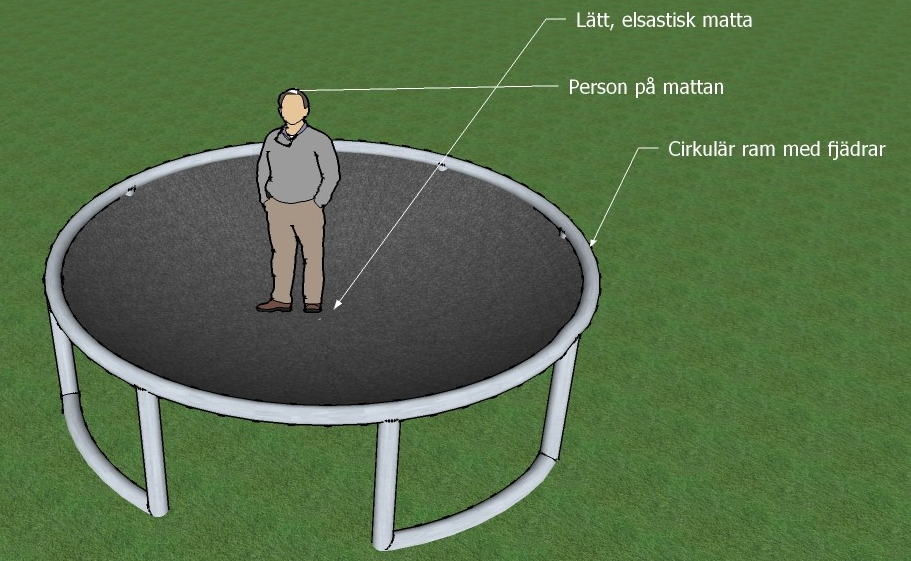
\includegraphics[scale=0.8]{Bild2}
\end{figure}
\clearpage

Figur 1 ger en mycket enkel överblick av vårt system. Studsmattan är helt cirkulär och har fjädrar som sitter radiellt från kanten riktade in mot mitten symmetriskt runt om hela cirkeln. Vi gör antagandet att personen som hoppar står precis i mattans mitt med fötterna tätt ihop.


Insignalen i vårt system blir alltså kraften som den hoppande personen utför på systemet då denne böjer eller sträcker på benen. Utsignalen i systemet definieras som mattans ändring i höjdled med referenspunkt i jämviktsläget på studsmattan.
%Uppdatera till att matcha den slutliga referensbilden
Krafterna uttryckta med pilar i bilden är gravitationskraften från massan $F_g$, fjäderns motkraft på massan $F_f$ och kraften från personen som trycker emot $F_a$.

Då fjädrarna i vår studsmatta är placerade symmetriskt och personen står placerad i mitten av mattan kan vi idealisera systemet som en enda fjäder verkande i y-led, eftersom de radiella krafterna tar ut varandra i symmetrin.

\subsection{Gravitationskraften $F_g$}

\begin{equation}
F_g = mg
\end{equation}
Gravitationskraften $F_g$ är den kraften som påverkar en massa $m$ med en konstant gravitationsacceleration $g$. 

\subsection{Fjäderkraften $F_f$}

\begin{equation}
F_f = -k(y - y_0)
\end{equation}
Fjäderkraften $F_g$ är den kraft som motverkar en fjäders avskiljning ifrån sitt jämviktsläge $y-y_0$, beroende på fjäderns i fråga fjäderkonstant $k$. Denna kraft är motriktad den av gravitationen. Sambandet har namnet Hookes lag.

\subsection{Dämpningskraften $F_d$}
\begin{equation}
F_d = -cv
\end{equation}
Dämpningskraften $F_d$ är den kraft som motverkar rörelsen i ett svängningssystem där $v$ är objektet i rörelses momentana hastighet och $c$ är dämpningskoefficienten för svängningsrörelsen. Denna kraft är motriktad den av gravitationen.

\subsection{Slutgiltig differentialekvation}

Systemet består av de åvanstående tre krafterna samt insignalen som alla är krafter i y-led. Vi vet att dessa krafter kommer att ta ut varandra eftersom alla krafter har en motsvarande lika står motriktad kraft. Vi får den totala kraften $F_{tot}$

\begin{equation}
F_{tot} = 0 = x(t) + F_g - F_f - F_d \leftrightarrow x(t) = F_g - F_f - F_d 
\end{equation}

Om vi ersätter krafterna med de ekvationer vi tog fram tidigare får vi

\begin{equation}
x(t) = F_g - F_f - F_d \leftrightarrow x(t) = m*\frac{d^2y}{dy^2} + c*\frac{dy}{dt} -ky(t)
\end{equation}

\newpage

\begin{thebibliography}{9}

\bibitem{sune2000}
  Sune Söderkvist,
  \emph{Tidskontinuerliga Signaler \& System}.
  \linebreak
  Erik Larsson AB, Linköping,
  3e upplagan,
  2000.

\end{thebibliography}

\end{document}